\documentclass[]{article}
\usepackage[]{algorithm2e}
\usepackage{amsmath}
\usepackage{framed}
\usepackage{tabularx}
\usepackage[dutch]{babel}
\usepackage{graphicx}
\usepackage{epstopdf}

%opening
\title{Practicum NMB : Eigenwaardenproblemen}
\author{Matthijs van Keirsblick en Harald Sch\"{a}fer}
\date{vrijdag 25 april 2014}

\newcommand{\opgave}[1]{\section*{Opgave #1}}


\begin{document}

\maketitle
\opgave{1}

We beginnen door een QR-factorisatie te berekenen van $A_{0}$ met eender welke methode. Vervolgens berekenen we $b = Q^{*}*b_{0}$. Met deze waarden kunnen we de iteratieve berekening starten die hieronder beschreven staat. De $G_{x}$ matrices zijn givens transformaties om de toegevoegde rijen van K terug op nul te stellen om zo terug een bovendriehoeksmatrix R te bekomen waarin de nieuwe waarden in verwerkt zijn.

\begin{framed}
\begin{algorithm}[H] 
 $Q^{(0)}*R^{(0)} = A_{0}$\\
 $b = Q^{(0)*}*b_{0}$\\
 \For{i = 1 to k}{
  $f = n*d$\\
  $R^{(i)} = G_{f}^{*}*...*G_{1}^{*}*
  \begin{bmatrix}
    	R^{(i-1)}	\\
    	K
    \end{bmatrix}$\\
  $R^{(i)} = R^{(i)}(:n,:)$\\
  $Q^{(i)} = I*G_{1}*...*G_{f} $\\
  $b^{(i)} = Q^{(i)*}*
  \begin{bmatrix}
      	b^{(i-1)}	\\
      	c
      \end{bmatrix}$\\
  $b^{(i)} = b^{(i)}(:n,:)$\\
 }
 
% \caption{How to compute incremental least squares solution with QR factorisation}
\end{algorithm}
\end{framed}

Aan het einde van elke iteratie is het mogelijk om $x^{(i)}$ te berekenen door achterwaardse substitutie toe te passen op de vergelijking $R^{(i)}*x^{(i)} = b^{(i)}$. Omdat na elke iteratie maar $R^{(i)}$ en  $b^{(i)}$ opgeslagen moet worden is het duidelijk dat het gebruikte geheugen niet toeneemt. Omdat de grootte van de matrices R en b niet toeneemt neemt het rekenwerk ook niet toe met elke iteratie. Voor het berekenen van een Givens-transformatie zijn 2 delingen, 2 vermenigvuldigen, een optelling en een vierkwantswortel nodig. Er moeten n*d Givens-transformaties berekend worden per iteratie. Een vermenigvuldiging met een rotatiematrix van grootte n+d zoals in dit geval vraagt 4*(n+d) vermenigvuldigingen en 2*(n+d) optellingen. Er gebeuren 2*n*d -1 van die matrix vermenigvuldiginge per iteratie. Tot slot  gebeurt er nog voor de berekening van de $b^{(i)}$ een matrix vermenigvuldiging waarvoor $(n+d)^2$ vermenigvuldigingen gebeuren en $(n+d-1)^2$ optellingen.

\begin{itemize}
  \item $n*d*2$ delingen
  \item $n*d$ vierkantswortels
  \item $n*d*2 + 2*(n+d)*(2*n*d-1) + (n+d-1)^2 \approx 4*n^2*d$ optellingen
  \item $n*d*4 + 4*(n+d)*(2*n*d-1) + (n+d)^2 \approx 8*n^2*d$ vermenigvuldigingen
\end{itemize}

%\section{}

\opgave{3}
Alvorens de QR methode, al dan niet met shifts, toe te passen op de matrix, moeten we hem omzetten naar Hessenberg vorm. Deze omzetting kost ons \'{e}\'{e}nmaal \textit{O}($n^3$) rekenwerk. \linebreak
Omdat de Hessenberg vorm al bijna bovendriehoeks is, kan de QR factorisatie in minder stappen uitgevoerd worden, namelijk in \textit{O}($n^2$) in plaats van in \textit{O}($n^3$). Deze factorisatie moet in iedere iteratie van de QR methode uitgevoerd worden, dus  de vermindering in rekenwerk is erg significant. 

\begin{figure}
\begin{center}
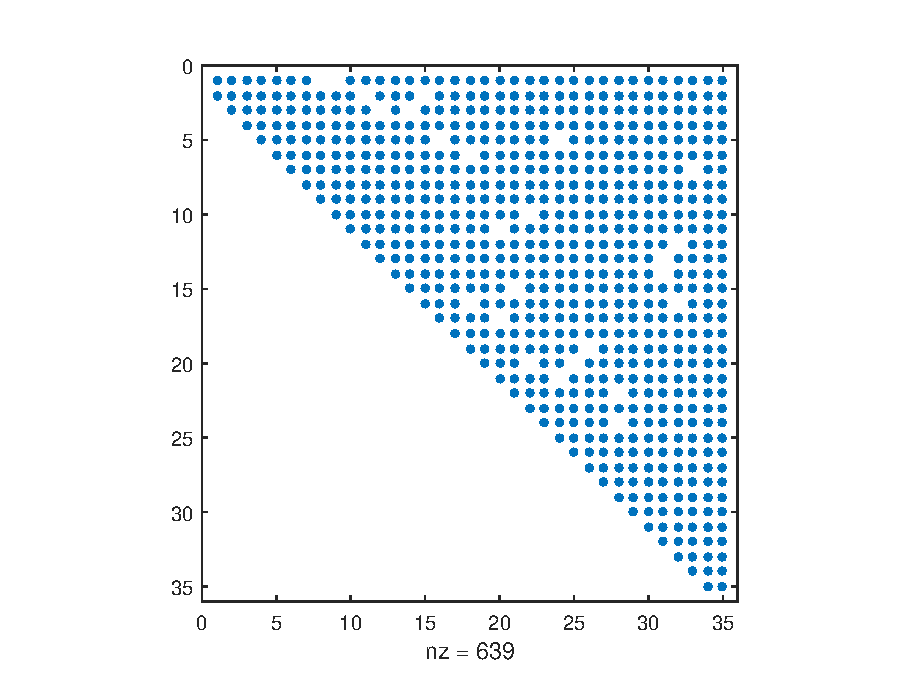
\includegraphics[width=1.4\textwidth]{opgave3.eps}
\end{center}
\caption{De structuur van de Hessenberg- vorm van mat1}
\end{figure}

\opgave{4}

De verwachting vanuit de theorie is dat de QR methode zonder shifts traag convergeert, zoals power- iteratie. De QR methode met shifts zou in het slechtste geval niet(Rayleigh shifts) of kwadratisch (Wilkinson shifts) convergeren. Hieronder worden het benodigde aantal iteratiestappen per methode in grafiek- en tabelvorm weergegeven, samen met de fout op het tussenliggende resultaat. We merken op dat  zowel de Rayleigh Shift als de Wilkinson Shift zorgen voor een kubische convergentie (aantal beduidende cijfers $* 3$ in iedere stap). 
De Wilkinson Shift heeft in dit geval een snellere convergentie door een (toevallig) goedgekozen eerste shiftwaarde. De convergentiefactor voor de eerste stap van de Wilkinson shift methode is hier $3.46$, voor de Rayleigh shift methode is hij $2.827$ en voor de QR methode zonder shift is hij zelfs kleiner dan 1. Het valt op dat de QR methode zonder shift niet lijkt te convergeren op deze grafiek. Dit is wel zo, maar pas na een groot aantal stappen (niet weergegeven). Na ~40 iteratiestappen is de machinenauwkeurigheid bereikt. 

\begin{figure}
\begin{center}
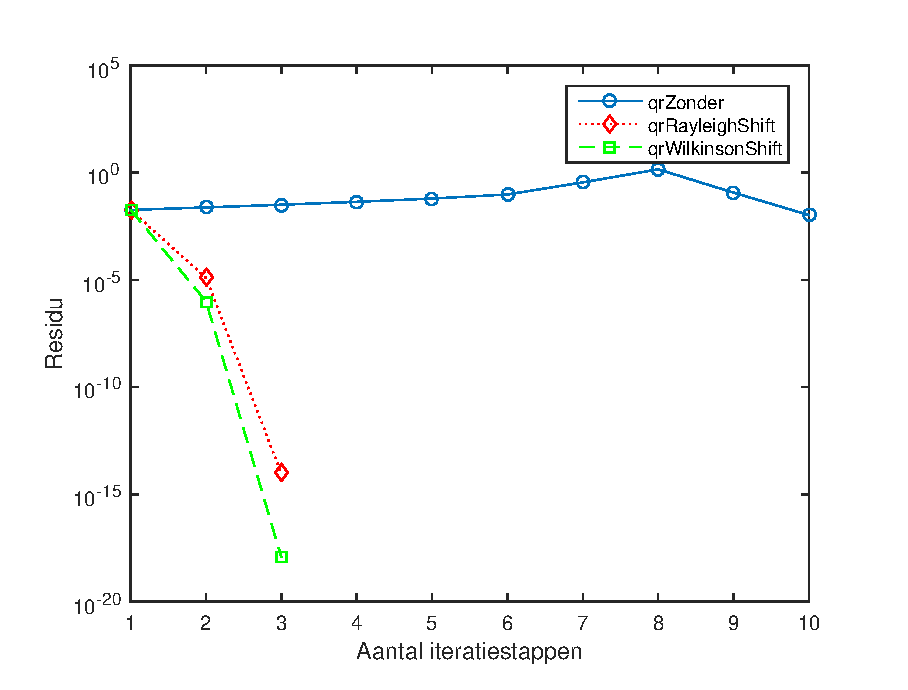
\includegraphics[width=1.4\textwidth]{opgave4.eps}
\end{center}
\caption{De fout op het berekenen van \'e\'en eigenwaarde.}
\label{figuurtje}
\end{figure}

\begin{table}
\noindent\makebox[\textwidth]{%
\begin{tabularx}{1.3\textwidth}{l|llllllllll}
Methode&1&2&3&5&10&20&25\\\hline
QRzonder&$0.01836$ & $0.02411$ & $0.03212$ & $0.06223$ & $0.0106$ & $1.498\times 10^{-6}$ & $2.059\times 10^{-8}$ \\
QRrayleigh & $0.01836$ & $1.234\times 10^{-5}$ & $9.558\times 10^{-15}$\\
QRwilkinson & $0.01836$ & $9.833\times 10^{-7}$ & $1.138\times 10^{-18}$   \\
\end{tabularx}}
\caption{convergentie QR methodes voor eigenwaardenberekening}
\label{tabelOpgave4}
\end{table}

Een aantal zaken zijn nog op te merken:
\begin{itemize}
	\item Voor de 2 methoden die gebruik maken van shifts, wordt in iedere stap een aantal keren een geshifte inverse iteratie gedaan, om zo het element op positie $(k,k)$ te laten convergeren naar de $k-de$ eigenwaarde. Opmerkzaam is dat de $i-de$ eigenwaarde met $i = 1,\dots,k-1$ als k het aantal eigenwaarden is dat we nog moeten berekenen, ook al genaderd wordt, terwijl het algoritme nog bezig is eigenwaarden verderop in de matrix te berekenen m.b.v shift- iteraties. Hoe kleiner i, hoe minder sterk dit effect. De oorzaak hiervan is dat de QR methode, naast inverse iteratie, ook simultane iteratie toepast.
	\item De methode met Wilkinson- shifts doet er 66 stappen over om alle eigenwaarden van mat1 te vinden tot op machineprecisie. De methode met Rayleigh- shifts doet er 83 stappen over, en die zonder shifts maar liefst 686 stappen. Wilkinson shifts zijn beter dan de Rayleigh shifts, omdat zij rekening houden met het symmetrische eigenwaarden. Rayleigh shifts kunnen in zo'n gevallen zorgen voor een trage (of zelfs onbestaande) convergentie.
\end{itemize}


\end{document}
